\chapter{Analyse du mouvement capturé}
Dans ce chapitre, nous explorons les différentes manières d'analyser le mouvement. En particulier, l'analyse du mouvement humain, dans le contexte d'un apprentissage ou de l'amélioration d'un geste, a principalement deux objectifs non exclusifs : (i) l'apprentissage ou l'amélioration du geste en lui-même, par imitation d'une succession de postures dans le temps ou par reproduction de ses principales caractéristiques (extraites de manière automatique ou non) et (ii), l'apprentissage ou l'amélioration de propriétés du ou des objets manipulés par l'intermédiaire du geste appris (manipulation d'un scalpel lors d'une procédure chirurgicale, par exemple).

L'apprentissage du geste par observation et imitation de démonstrations peut être qualifié de naturelle, simple à mettre en œuvre mais peu efficace sans un grand nombre d’itérations du processus « démonstration-imitation » \parencite{Yang2014RoP}. Le savoir de l'expert permet le plus souvent de juger de la qualité du geste effectué. Ce regard expert sur le geste peut conduire à des propositions d'améliorations, sous la forme d'entraînements relatifs aux défauts du geste effectué. Les observations et l'analyse de l'expert sont cependant limitées par la complexité du geste : un geste qui fait intervenir, rapidement, de nombreuses parties du corps peut être difficile à analyser dans son intégralité, comme pour la danse par exemple \parencite{Kyan2015ABD}. Il est possible de pallier cette difficulté en analysant le mouvement capturé. En effet, l'utilisation de données de mouvements capturés permet d'avoir une représentation visualisable à volonté, selon différentes vitesses de lecture, sous différents angles de vue \parencite{Yoshinaga2015Doa} et permet également d'utiliser des processus automatiques afin d'aider cette analyse à l'aide de : calculs de descripteurs, détections d'une séquence ordonnée d'actions, l'utilisation de techniques d'apprentissage automatique ou la réduction des données. Les parties suivantes présentent différentes méthodes existantes pour l'analyse des gestes tout en positionnant l'usager et ses contributions (apprenant ou enseignant) au sein de chacune d'elle. Ces catégories ne sont pas exclusives, c'est-à-dire qu'un même système dédié à l'apprentissage de mouvement peut se trouver à l'intersection de deux catégories ou plus.

\section{Analyse du geste par observation humaine}
Cette section présente plusieurs études où l'analyse du geste est faite de manière empirique par un humain. Cette analyse peut directement s'effectuer par visualisation du mouvement, ou à l'aide de métriques calculées en fonction des besoins d'observations. Dans les deux cas, les données doivent être analysées par un humain dans un premier temps et les retours sont systématiquement délivrés par un expert à un apprenant.

Le domaine médical est un domaine qui nécessite non seulement de pouvoir étudier la motricité du patient, mais aussi son état physiologique. À l'aide d'un ensemble de capteurs hétérogène (réduit \parencite{Alankus2010TCG} ou non \parencite{deVries2006Cro}), il est possible d'obtenir suffisamment d'informations pour que le médecin soit capable de délivrer un verdict. Bien que de nombreux types de capteurs existent pour l'analyse médicale, nous nous concentrons ici sur les capteurs permettant d'obtenir des données relatives aux mouvements, et non des indications sur l'état physiologique du patient (capteur cardiaque, par exemple).

L'analyse de la démarche fait un usage intensif des données de mouvements capturés \parencite{Chen2016TPG}. Cette analyse permet d'évaluer le résultat de nombreuses procédures médicales chez un patient : pose de prothèse, chirurgie, rééducation, mais également le suivit de l'évolution de la posture, ainsi que les risques de chute, notamment chez les personnes âgées. Ainsi, il est crucial d'obtenir des données correspondant aux besoins d'observation et d'analyse des médecins (Fig. \ref{fig:gait_possibilities}). De tels descripteurs peuvent être extraits à partir d'un squelette 3D.

\begin{figure}
    \centering
    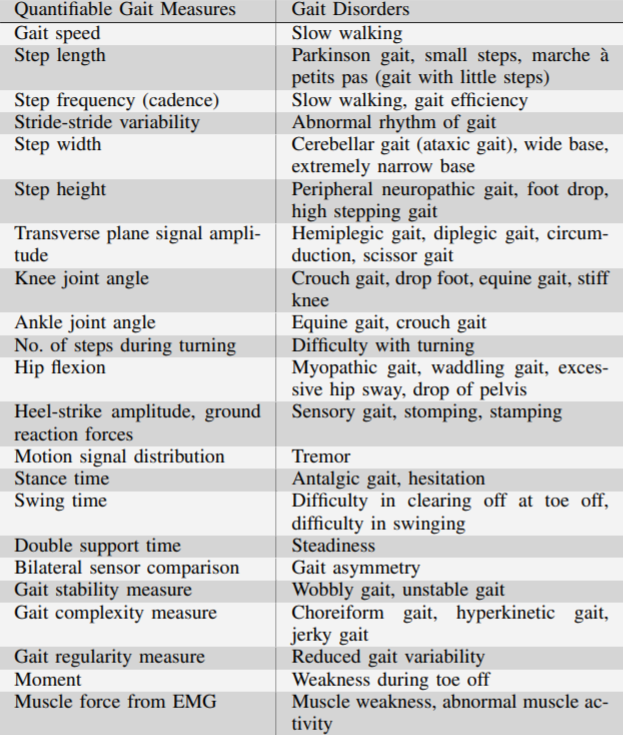
\includegraphics[width=9cm]{pictures/gait_possibilities.png}
    \caption[Descripteurs pour l'analyse de la démarche \parencite{Chen2016TPG}]{Des exemples de descripteurs extractibles relatifs à la démarche possible et leurs applications pour la détection de pathologies \parencite{Chen2016TPG}.}
    \label{fig:gait_possibilities}
\end{figure}

La chirurgie gagne beaucoup à utiliser les casques de réalité virtuelle afin de simuler des procédures dans un environnement clinique d'apprentissage. En effet, il n'est pas envisageable de s'entraîner sur de vrais patients \parencite{Kneebone2004Sac}. Ainsi, l'utilisation d'environnements virtuels, combinés par exemple à des processus de gamification \parencite{Pulijala2017VRS}, permet d'entraîner plus de chirurgiens en parallèle, ainsi que de permettre une vérification des acquis sans risque. Dans les travaux de Choi \textit{et al.} \parencite{Choi2015103}, l'utilisation conjointe de retours visuels en temps réel, ainsi que d'indicateurs calculés par rapport à la tâche à effectuer (temps de la procédure, force appliquée, etc.) permet de proposer une visualisation de la performance.

Le sport est un domaine où l'apprentissage du geste est au coeur de la formation. Il est nécessaire de pouvoir évaluer à la fois le résultat du geste, mais également la manière dont il est fait, afin d'éviter des risques de blessure \parencite{Rawashdeh2016WIMU}. L'utilisation d'experts virtuels est une des possibilités offertes par la capture de mouvements. Bien que ces systèpmes permettent parfois de s'affranchir de la présence d'un expert, ils ne présentent pas systématiquement une amélioration de l'apprentissage par rapport aux méthodes d'enseignement traditionnelles \parencite{Philo2003Tfp}.

Pour l'apprentissage du karaté, le système développé par Burns \textit{et al.} propose un environnement en réalité virtuelle \parencite{Burns2011Uvh}. L'apprenant doit, au fur et à mesure des séances, reproduire à l'identique les gestes de l'expert. Les sessions sont divisées en deux parties : une partie sur l'explication du geste à effectuer, fournie à l'aide d'une vidéo de l'expert effectuant le mouvement et une autre sur des exercices relatifs au geste. L'expert y est représenté sous forme 3D dans un environnement virtuel correspondant à un dojo (Fig. \ref{fig:Burns_karate}). L'évaluation est réalisée par l'expert, une fois au début de l'apprentissage et une fois à la fin, en analysant les vidéos des gestes des apprenants. Ces enregistrements sont réalisés hors du contexte virtuel. L'expert évalue les gestes des apprenants en attribuant un score, en fonction du degré de similitude du geste de l'apprenant par rapport à celui de l'expert. Les résultats montrent que l'avatar virtuel est aussi efficace qu'un expert réel pour l'apprentissage de ces gestes.

\begin{figure}
    \centering
    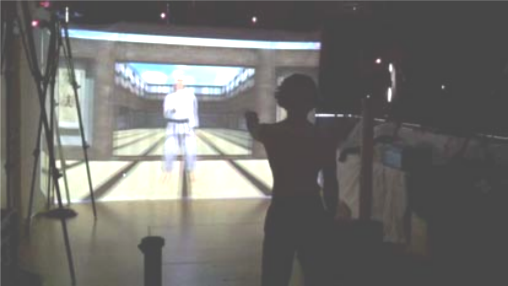
\includegraphics[width=\textwidth]{pictures/Burns_karate.png}
    \caption[Environnement virtuel pour l'apprentissage du karaté \parencite{Burns2011Uvh}]{L'environnement virtuel pour le Karaté proposé par Burns \textit{et al.} est utilisé pour l'entrainement de l'apprenant. L'évaluation est faite de manière qualitative par un expert \textit{a posteriori} \parencite{Burns2011Uvh}.}
    \label{fig:Burns_karate}
\end{figure}

Le système développé par Le Naour \textit{et al.}, présenté dans le chapitre 2, permet d'aider à l'apprentissage de mouvement en superposant le modèle de l'expert à celui de l'apprenant au sein d'un environnement virtuel \parencite{LeNaour2019S3V}. Le cas de test utilisé était celui du lancer au football américain. À partir d'une démonstration effectuée par l'expert, l'apprenant doit ensuite effectuer une suite de plusieurs lancers, à partir desquels sont calculés la valeur de l'écart-type du \textit{DTW} entre les mouvements de l'apprenant et de l'expert, ainsi que la distance du lancer par rapport au centre de la cible visée. Le groupe ayant reçu la visualisation du mouvement de l'apprenant superposé à celui de l'expert comme retour a montré une amélioration plus importante du geste que les groupes ne l'ayant pas obtenu.

À l'inverse, Kora \textit{et al.} ont proposé un environnement en réalité augmentée permettant l'apprentissage du golf en autonomie \parencite{Kora20151559}. La projection du modèle de l'expert dans un casque porté par l'apprenant, superposé au squelette (capté à l'aide d'une Kinect) de la personne faisant le geste, permet d'aider l'apprenant à corriger son geste au fur et à mesure de l'entraînement. L'apprenant est en auto-évaluation : aucune indication ne lui est fournie, c'est donc à lui d'être capable d'évaluer seul les changements à apporter à son geste afin de parfaire le mouvement du swing.

Des systèmes se basent sur la superposition des données de l'apprenant avec celles des experts afin de proposer une correction par mimétisme \parencite{Yoshinaga2015Doa}. Dans ces cas, le mouvement de l'apprenant est rejoué par dessus celui de l'expert, et les corrections peuvent s'effectuer par rapport au décalage temporel ou spatial de l'apprenant par rapport à l'expert.
Le système proposé par Yoshinaga et Soga, testé sur l'archerie japonaise, permet d'agréger plusieurs modèles experts afin de proposer soit un expert au choix, soit l'expert le plus proche de l'étudiant morphologiquement parlant, soit une moyenne des experts ou soit l'expert médian (c'est-à-dire l'expert le plus proche de la moyenne des experts) \parencite{Yoshinaga2015Doa}. Cette approche permet de limiter les différences morphologiques, dans le cas où un des modèles experts est semblable à celui de l'apprenant. La comparaison du geste de l'apprenant à celui de l'expert est réalisée à l'aide d'une correspondance en programmation dynamique : ainsi, le mouvement est représenté de façon amorphologique, et il est possible de faire correspondre les mouvements temporellement, même en présence de variations de timing, vitesse et d'amplitude des mouvements. Il est possible d'utiliser ce système soit en autonomie, soit à l'aide d'un expert qui analysera le geste de l'apprenant. Dans ce cas, l'expert peut être en mesure d'expliquer les différences entre le geste de l'apprenant et celui des modèles d'experts, ajoutant ainsi son expertise au retour visuel (Fig. \ref{fig:Yoshiniga_archery}).

\begin{figure}
    \centering
    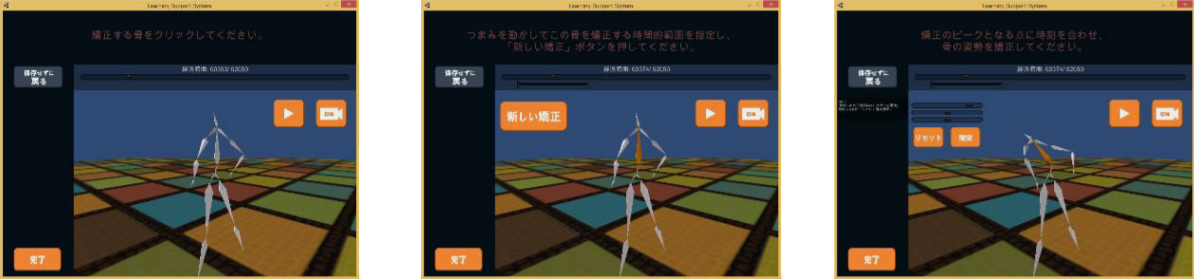
\includegraphics[width=\textwidth]{pictures/Yoshiniga_archery.png}
    \caption[Correction du mouvement de l'apprenant \parencite{Yoshinaga2015Doa}]{L'environnement proposé par Yoshinaga \textit{et al}. permet à l'expert de modifier directement les positions et les orientations des membres du corps de l'apprenant sur l'enregistrement du geste originel, afin de lui proposer des corrections à distance \parencite{Yoshinaga2015Doa}.}
    \label{fig:Yoshiniga_archery}
\end{figure}



\section{Analyse par observation d'indicateurs calculables du geste}
L'explication des caractéristiques d'un geste, ainsi que son évaluation, peut varier en terme de précision, en fonction du contexte applicatif mais également de la possibilité d'expliciter et de formaliser les caractéristiques importantes en descripteurs calculables. Dans le cas où les caractéristiques du geste à réaliser, ainsi que les propriétés biomécaniques associées, sont connues à l'avance, il est possible de proposer des valeurs précises pour les différentes caractéristiques des différents mouvements à effectuer pour chaque partie du corps concernée, et ainsi permettre de fournir, par exemple, une amplitude acceptable, un intervalle de déplacement correct, une rotation cible, etc. Dans ces cas, l'analyse automatique du geste est possible à condition que ces quantités puissent être mesurées ou calculées à partir des données capturées. Deux grandes stratégies non-exclusives d'analyse automatique peuvent s'appliquer : l'analyse automatique des caractéristiques du geste en lui-même, et l'analyse automatique de la position d'un objet au cours du temps, permettant ainsi de donner des pistes quant aux conseils à donner à l'apprenant.

Dans ce dernier cas, les outils utilisés pour simuler les objets réels peuvent être multiples. L'utilisation de dispositifs haptiques est courante dans le domaine de la chirurgie. La simulation d'outils (trocarts, scalpels, sondes, etc.) intégrés dans des scènes virtuelles réalistes permet de s'entrainer à pratiquer des opérations chirurgicales dans des conditions proches d'une situation \textit{in vivo}.

Pham \textit{et al.} s'intéressent à la position d'un forceps au cours d'une simulation d'un accouchement, et plus particulièrement la trajectoire de la position et celle de l'orientation. Ils comparent celles de l'objet manipulé par l'apprenant par rapport à celles de l'objet manipulé par l'expert \parencite{Pham2010Tdg}. La corrélation entre les signaux correspondants aux trajectoires de l'expert et de l'apprenant est calculée, et sa valeur est utilisée en tant que score, qui correspondant à la similitude entre ces trajectoires. Despinoy \textit{et al.} proposent une approche qui analyse également la position et l'orientation d'un porte-aiguilles au cours d'une opération de réalisation de points de suture \parencite{Despinoy2016UTS}. Le mouvement est segmenté en plusieurs parties grâce aux points d'inflexion de la trajectoire de l'outil considéré. Ces points correspondent aux moments où le geste subit un changement brusque, soit dans sa linéarité, soit dans sa direction.

Dans le cadre du suivi des patients atteints de la maladie de Parkison, le système développé par Wang \textit{et al.} permet, à l'aide d'un seul capteur et d'une suite de mouvements à réaliser par le patient, de proposer aux médecins des données permettant d'évaluer la progression de la maladie \parencite{Wang2013HMM}. L'expérimentation proposée cherche à observer et quantifier la dégradation de la posture et des mouvements due à la maladie de Parkinson, à l'aide de la distance faite à chaque pas, le balancement de la posture, le degré de balancement des bras et la constance de l'intervalle de temps entre chaque pas. Ces données étaient relevées au cours de deux mouvements à réaliser par les patients : (i) marcher et (ii) s'asseoir et se lever. La succession de mouvements à réaliser permet aux médecins de vérifier l'état d'avancement de la maladie, et le système permet de faire un suivi à distance, et ainsi d'éviter les déplacements des patients. L'objectif du système n'est cependant pas de proposer une évaluation du geste, mais des métriques qui peuvent être utilisées par un médecin pour évaluer la progression de la maladie.

Le geste a une place prédominante dans l'apprentissage du sport. La technicité, ainsi que la précision des gestes à réaliser en font un domaine d'étude idéal pour le développement de systèmes d'analyse automatique. Au sein de ce domaine, deux cas d'étude principaux se dégagent : l'analyse du geste de l'apprenant en fonction de critères définis au préalable, ou la découverte de la différence entre les gestes experts et ceux des débutants.

Une première approche consiste à effectuer une analyse basée sur les positions relatives des parties du corps pour proposer une évaluation du geste. Yamaoka \textit{et al.} ont proposé un système qui évalue plusieurs modalités du lancer de disque, à différents moments du lancer (pré-lancer, lancer, post-lancer) (Fig. \ref{fig:flying_disc_TEL}) \parencite{Yamaoka2013FoF}. Le mouvement est segmenté selon ces catégories en observant et comparant les positions relatives de plusieurs articulations. Ainsi, pour un droitier, le geste est considéré comme faisant partie du pré-lancer tant que la position de la main est située à la droite de  celle du centre des épaules par rapport à l'axe horizontal. La période de lancer est celle où la position de la main, toujours selon le même axe, est située entre le centre des épaules et le coude droit. Le post-lancer commence à partir du moment où la main droite est à gauche du coude droit. L'évaluation du geste se fait selon 5 critères :
\begin{itemize}
	\item la présence d'une phase d'élan avant le geste
	\item l'élévation de la main par rapport à l'épaule
	\item le changement de hauteur de la main au cours du lancer (afin que le disque reste parallèle au sol durant le vol)
	\item l'angle formé par le triplet d'articulations épaule/coude/poignet
	\item la rotation des hanches lors du lancer
\end{itemize}

En vérifiant que chacune de ces modalités respecte un intervalle ou ne dépasse pas un seuil spatial, le système est en mesure de donner un retour à l'apprenant. Ce retour est donné en temps réel, et il n'est pas possible de rejouer le mouvement ni de visualiser les conseils antérieurement : l'impact sur l'apprentissage s'en trouve diminué.

\begin{figure}
    \centering
    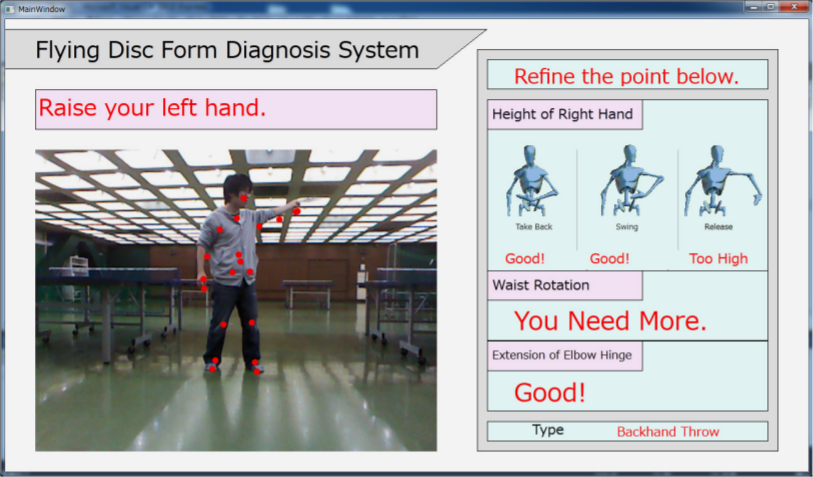
\includegraphics[width=\textwidth]{pictures/flying_disc_TEL.png}
    \caption[Système d'apprentissage du lancer de disque \parencite{Yamaoka2013FoF}]{Le système développé par Yamaoka \textit{et al.} pour l'apprentissage du lancer de disque. Les conseils sont donnés sur plusieurs caractéristiques du geste en même temps \parencite{Yamaoka2013FoF}.}
    \label{fig:flying_disc_TEL}
\end{figure}

Comme présenté précedemment, les travaux de Morel proposent l'extraction de descripteurs du mouvement dans le cadre de l'analyse de la performance sportive \parencite{Morel2017Mts}. Après un recalage spatial (à l'aide d'une transformation linéaire) et temporel (à l'aide de l'algorithme de la \textit{DTW}), les différences spatiales et temporelles entre le geste de l'apprenant et celui de l'expert sont données en calculant d'une part l'alignement spatial d'un membre par rapport au membre de référence, et d'autre part la différence entre les chemins de déformations induits par les alignements des membres de l'apprenant et de l'expert. Ces erreurs sont ensuite traduites en indications pour la position des membres au cours du mouvement.


Le système de Makio \textit{et al.} propose une autre stratégie en se basant sur la trajectoire et la vitesse du poignet lors d'un service au tennis, afin de mettre en lumière les différences entre les gestes des experts et ceux des débutants \parencite{Makio2007DoS}. L'analyse se base sur une extraction des règles d'associations entre les différentes parties du corps, à partir desquelles sont extraits des motifs fréquents. La distance entre ces motifs est calculée à l'aide d'une distance euclidienne. Bien que cette analyse permette de mettre en évidence les différences entre les gestes de l'expert et ceux de l'apprenant, et propose également une visualisation des trajectoires de l'expert et de l'apprenant, aucun conseil n'est ensuite donné par le système.

Dans le domaine de la danse, le système proposé par Maes \textit{et al.} permet d'apprendre le geste en trois étapes : la démonstration, l'apprentissage et l'évaluation ludifiée \parencite{Maes2012DtM}. L'étape de démonstration permet à l'expert de s'enregistrer, tout en configurant plusieurs options telles que la musique, le tempo, le nombre de pas par figure de danse, le nombre d'entraînements requis, \textit{etc.} L'apprentissage se base sur la reproduction des pas effectués par le modèle de l'expert, autant sur l'aspect spatial que temporel, accompagné par les schémas des différents déplacements et rotations à effectuer. Dès cette étape, la corrélation entre le modèle de l'expert et la performance de l'apprenant est calculée, afin de fournir un premier retour sur la performance de ce dernier, à l'aide du coefficient de corrélation croisée de Pearson, calculé sur les données de mouvement de l'expert. Enfin, la partie d'évaluation propose à l'apprenant de danser et effectue une comparaison, toujours selon le même critère, des différents mouvements constituant la danse, permettant ainsi l'évaluation sous la forme d'un score à maximiser. Cette méthode passe cependant outre les spécificités de chaque partie du corps et ne propose qu'une évaluation globale du mouvement, ce qui résulte en une perte d'informations, notamment au niveau des défauts ponctuels du geste.

Toujours dans le domaine de la danse, Kyan \textit{et al.} ont développé un système utilisant la réalité virtuelle afin de faciliter l'évaluation de la performance de l'apprenant \parencite{Kyan2015ABD}. En utilisant un unique descripteur, à l'aide d'une projection dans un espace sphérique des mouvements de danse, le mouvement est décomposé en plusieurs parties. Chacune de ces parties est ensuite comparée à une base de données de composants gestuels d'expert réalisés au préalable. Cette décomposition permet d'estimer quel mouvement était en train d'être réalisé par l'apprenant. Une fois que le mouvement est reconnu, une comparaison entre des descripteurs angulaires extraits permet de donner un score pour chaque partie du mouvement de danse. Ce score est calculé en fonction de la distance euclidienne entre les signaux de l'apprenant et de l'expert, après alignement temporel à l'aide de l'algorithme du DTW. Une autre partie de ce système permet également de superposer le modèle de l'apprenant à celui de l'expert, afin de corriger précisément la position de chaque partie du corps concernée. L'évaluation conduite montre que le mouvement est correctement segmenté par le système ; cependant, la visualisation des mouvements ne permet qu'une faible amélioration de la performance de l'apprenant. De plus, aucun alignement morphologique, spatial ni temporel n'est effectué.

\begin{figure}
    \centering
    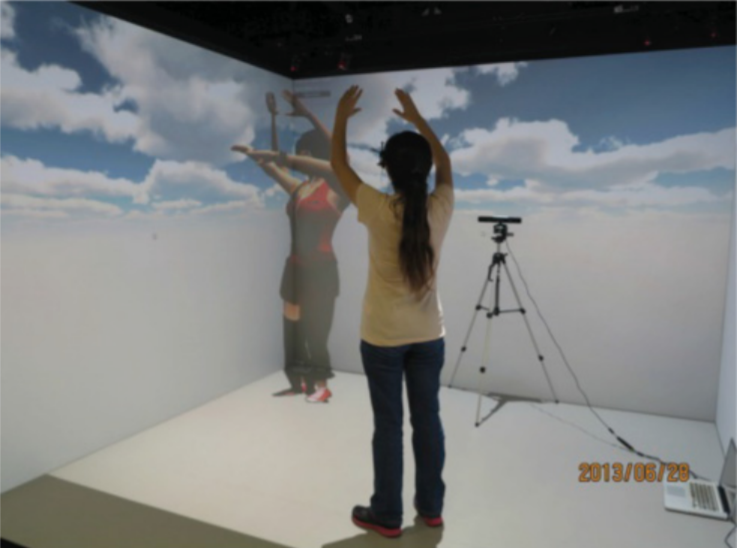
\includegraphics[width=\textwidth]{pictures/dance_cave_TEL.png}
    \caption[Système d'apprentissage de mouvement utilisant un CAVE pour la captation et la comparaison \parencite{Kyan2015ABD}]{Le système développé par Kyan \textit{et al.} fait usage de la réalité virtuelle dans un système CAVE afin de proposer soit une observation côte à côte des mouvements de l'expert et de l'apprenant, soit superposée (cas de l'image) \parencite{Kyan2015ABD}.}
    \label{fig:dance_cave_TEL}
\end{figure}

Toujours dans le domaine des arts, l'analyse des efforts réalisés par les joueurs de violon est le sujet d'étude de Rasamimanana et Bevilacqua\parencite{Rasamimanana2008EbA}. À partir d'informations cinématiques provenant du geste de la personne, telles que : la vitesse, le tremblement (\textit{jerk}) et l'impulsion (du mouvement), il est possible de déterminer quel a été le mode de jeu utilisé par la personne réalisant le geste : \textit{détaché} ou \textit{martelé}.

Les systèmes calculant des indicateurs à partir du geste de l'apprenant permettent, dans une certaine mesure, de s'affranchir de la présence de l'expert pour l'évaluation et la restitution des conseils à l'apprenant. Leur objectif est souvent de proposer une évaluation de manière automatique, sans nécessiter l'intervention d'un expert pour interpréter les données. La connaissance experte doit être intégrée \textit{a priori}, dès la phase de conception. Dans ce contexte, la généricité des descripteurs extraits n'est pas assurée si elle n'est pas considéré dès la conception du système, et le système n'est souvent pas réutilisable dans des contextes différents. De plus, les retours données prennent le plus souvent la forme d'un score à maximiser (indiquant généralement la proximité des données de l'apprenant à celles de l'expert), qui, bien que facilement interprétable en terme de qualité du geste effectué, ne permet pas systématiquement de fournir des indications quant aux améliorations à apporter au geste.


\section{Analyse par détection d'une séquence ordonnée d'actions}
Dans les systèmes d'apprentissage du geste, l'analyse peut se focaliser sur la suite d'actions à réaliser afin d'atteindre l'objectif. Dans ce cas, le geste est décomposé en unités considérées comme élémentaires par le système afin de représenter chaque action. La granularité des unités élémentaires est dépendante du système considéré. Ainsi, il est possible de comparer cette suite de mouvements de manière ordonnée à l'enchainement attendu par l'expert.

%Dans ces travaux, on retrouve les études qui s'intéressent à la manipulation d'objets. Ainsi, dans les travaux de Toussaint, à partir de traces hétérogènes (manipulation d'un objet simulant un trocart, mais également position du regard) et d'un ensemble de séquences à réaliser prédéfinies par un expert, l'objectif est de permettre à la fois l'évaluation des connaissances de l'apprenant et de lui donner des retours en fonction du type de défaut présent au sein de la procédure. Le mouvement à reproduire est divisé en phases, chaque phase comprenant une suite de plusieurs actions. La finalité du système est de comparer la séquence d'actions (appelées « perceptivo-gestuelle », car combinant des données relatives au regard de l'apprenant et du mouvement de l'objet) aux séquences pré-définies par les experts \parencite{BMT_2015}. Bien qu'il existe un ordre précis pour les phases, déterminé à l'avance par l'expert, le système ne contraint pas l'ordre des phases de résolution de l'opération, c'est-à-dire que l'apprenant peut librement passer d'une phase à une autre au cours de l'opération. Cependant, ces changements de phases sont analysés par le système, et interprétés comme étant une erreur dans l'opération qui est constatée par l'apprenant. Le nombre de retours en arrière est corrélé à une faible maîtrise des connaissances à appliquer. Ainsi, il est possible d'évaluer à la fois si les gestes sont effectués dans le bon ordre, mais également si l'ordre des phases est correct. Cependant, le ou les gestes menant à la réalisation des actions ne sont pas directement évalués, l'analyse se focalisant sur la détection d'une suite ordonnée d'actions.

Mahdi \textit{et al.} ont développé un environnement virtuel permettant à n'importe-quel enseignant de définir lui-même ses scénarios d'apprentissage à partir de scènes virtuelles pré-existantes \parencite{Mahdi2019TaE}. L'objectif est de permettre de lier la description du scénario pédagogique aux activités de l'apprenant au sein de l'environnement virtuel. Chaque activité peut être divisée en une séquence d'actions, qui elles-mêmes peuvent être divisées en séquences de comportements élémentaires, appelées " Primitives Virtuelles de Comportement " : (i) observation du monde virtuel, (ii) déplacement dans le monde virtuel, (iii) interaction avec le monde virtuel et (iv) communication avec d'autres personnes ou avec l'application. Les activités sont réalisées par l'apprenant à l'aide d'objets d'intérêt auxquels ont été associés des propriétés techniques (position, forme, couleur, \textit{etc.}) ou pédagogiques (utiliser l'objet, verser, le bouger, \textit{etc.}). L'éditeur de scénario permet ainsi à l'expert de définir une suite d'activités lors de la conception du scénario. Les premiers tests à l'aide d'enseignants ont montrés que l'éditeur leur était utile, et permettait de générer des scénarios de manière aisée.

Les travaux de Delest \textit{et al.} ont mené à la création d'un système où l'expert peut lui-même proposer un parcours, personnalisable à l'aide de points de contrôle (\textit{checkpoints}), représentés sous la forme d'objets 3D simples (e.g. sphère, parallélépipède rectangle) à passer dans un ordre précis \parencite{Delest2019MaE} (Fig. \ref{fig:Delest_system}). Dans ce système, l'expert doit déterminer à l'avance si le parcours concerne le corps de l'apprenant (analyse de la démarche, par exemple) ou un objet présent au sein de la scène. Une fois l'objet d'intérêt choisi, l'expert place ensuite un point de contrôle de départ, possiblement des points de contrôles intermédiaires puis un point de contrôle d'arrivé. Il est possible de modifier la taille et la forme de ces points de contrôles, permettant ainsi de les adapter aux différents objets manipulables (Fig. \ref{fig:Delest_system} au milieu). L'expert doit ensuite réaliser le mouvement lui-même, afin de disposer d'un mouvement de référence (mouvement cible). Le mouvement est considéré comme validé lorsque l'objet ou la personne a franchi (c'est-à-dire qu'il y a collision entre le point de contrôle et l'objet ou la personne) tous les points de contrôle dans l'ordre. Le mouvement est ensuite segmenté en fonction des points de contrôle. Chaque mouvement est ensuite comparé au mouvement de référence réalisé par l'expert, selon plusieurs métriques : de manière globale à l'aide de l'algorithme du DTW, mais également à l'aide d'indicateurs cinématiques, tels que la vitesse, la saccade du mouvement (\textit{jerk}), \textit{etc.} (Fig. \ref{fig:Delest_system} à droite).

\begin{figure}
    \centering
    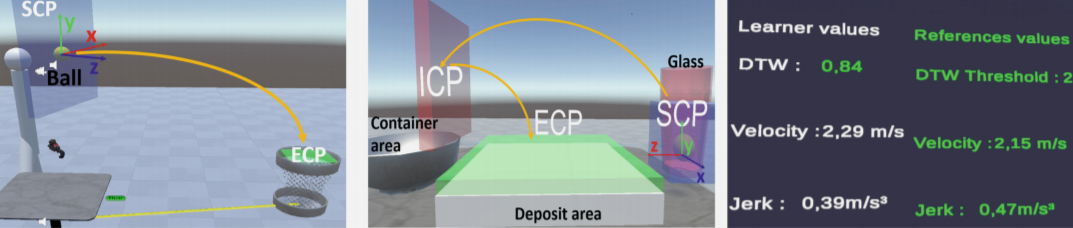
\includegraphics[width=\textwidth]{pictures/Delest_system.png}
    \caption[EVAH permettant de générer des parcours à suivre pour un objet ou l'apprenant \parencite{Delest2019MaE}]{Le système proposé par Delest \textit{et al.} permet à l'expert de générer un parcours à suivre, soit pour la personne, soit pour un objet, dans un ordre prédéfini, et propose l'affichage de plusieurs métriques permettant de comparer le geste de l'apprenant à celui de l'expert \parencite{Delest2019MaE}.}
    \label{fig:Delest_system}
\end{figure}

Dans ces systèmes, l'évaluation du geste est principalement centrée sur l'ordre dans lequel est réalisé un ensemble d'unités élémentaires, plutôt que sur l'évaluation en elle-même du geste sous-jacent à ces actions ou unités. Ainsi, les caractéristiques du geste ne sont pas systématiquement analysées (excepté pour \parencite{Delest2019MaE}). Lors de la manipulation d'objets, c'est l'état de l'objet à des moments clés du mouvement qui va être considéré. Dans ce cas, on considère que le geste qui a mené à l'état cible est correct, sans l'analyser en lui-même.

Ces systèmes fonctionnent par décomposition et analyse des unités élémentaires composant le geste initial. La nature de ces unités élémentaires (durée, granularité de la décomposition, \textit{etc.}) peut varier d'un système à l'autre. La finalité de cette décomposition est de comparer l'enchainement d'unités élémentaires à l'enchainement attendu par l'expert. Cela implique de disposer d'un modèle de connaissance du geste à effectuer, et son intégration se fait souvent dès la conception du système, ne permettant pas d'assurer sa généricité. Cependant, des systèmes tels que ceux développés par Delest \textit{et al.} \parencite{Delest2019MaE} et Mahdi \textit{et al.} \parencite{Mahdi2019TaE}, conçus afin être génériques au regard du geste à accomplir, permettent une ré-intégration de la connaissance experte aisée à l'aide d'un éditeur de scénarios pédagogiques intégrés au système. L'apprentissage se focalise néanmoins sur la suite d'action à réaliser, leur enchainement et la manipulation d'un objet, mais pas sur les gestes qui permettent d'arriver aux états ou à la succession de postures désirés.


\section{Analyse fondée sur des techniques d'apprentissage automatique}
Il est également possible d'utiliser des algorithmes d'apprentissage automatique afin d'analyser automatiquement le geste. Dans ce cas, les descripteurs extraits sont le plus souvent choisis en amont du processus d'analyse, puis utilisés dans un algorithme d'apprentissage automatique afin d'observer la similitude entre le mouvement et ceux présents au sein d'une base de données.

Par exemple, les travaux de Pirsiavash \textit{et al.} proposent une approche sur l'évaluation de geste sans \textit{a priori} sur le mouvement en lui-même \parencite{Pirsiavash2014AQA}. Les données sont extraites à partir de vidéos, et sont constituées de descripteurs variés, tels que des gradients de pixels, des vitesses et des trajectoires, ainsi que des postures successives réalisées par les sportifs. Cette étude se base sur les performances d'athlètes olympiques dans deux sports différents, la patinage artistique et le plongeon. Les données extraites sont ensuite associées à un score donné par des experts ; dans ce cas, il s'agit de scores donnés par les juges olympiques. L'étude montre que les juges donnent la même note dans 96\% des cas, ce qui suggère qu'il existe un socle de règles communes permettant l'évaluation. Les couples mouvements / score sont ensuite utilisés en entrée d'un SVM. L'algorithme a permis d'extraire les moments les plus déterminants dans l'attribution du score par les juges. Les scores donnés par l'algorithme sont comparés à ceux données par l'expert, à l'aide de la corrélation de Spearman. Les valeurs de ce coefficient montre que les scores donnés sont encore assez éloignés de ceux des experts. L'analyse permet néanmoins de mettre en évidence une évaluation de la qualité du geste supérieure à celle d'un non-expert du domaine.

Patrona \textit{et al.} utilisent des algorithmes de logique floue (\textit{fuzzy logic}) afin de proposer une segmentation, une reconnaissance et une évaluation de gestes \parencite{Patrona2018MaA}. Il n'y a pas d'\textit{a priori} sur les gestes pouvant être traités par le système. Dans cette études, les gestes considérés sont variés, tous pris au sein de bases de données : \textit{swing} au golf, taper dans ses mains, s'asseoir, lancer, service au tennis, \textit{etc.} Des descripteurs cinématiques sont extraits du mouvement, puis utilisés par des classifieurs binaires, chacun entrainé à reconnaître un mouvement spécifique. Une fois le mouvement reconnu par le système, la phase d'évaluation s'effectue entre le mouvement de l'apprenant et les mouvements cibles contenus dans la base de données de mouvements. Plusieurs étapes sont ensuite réalisées (Fig. \ref{fig:Patrona_motion_evaluation}) : alignement temporel des mouvements (apprenant et cible) à l'aide d'un algorithme de DTW multivarié, normalisation de la longueur des membres afin d'éviter les différences morphologiques, alignement spatial des mouvements à l'aide de la différence de rotation du corps calculée à partir de la position des épaules et du torse, puis utilisation des différences de positions et de vitesses entre les deux mouvements afin de proposer un retour à l'apprenant. Ces retours sont donnés sous la forme d'un score de similarité entre les mouvements (calculé à l'aide de l'algorithme du \textit{DTW}), mais également les parties du corps et les articulations les plus éloignées de celles de l'expert, au regard des descripteurs utilisés (positions et vitesses). Un exemple de retour donné par le système est le suivant :

\vspace{0.5cm}« The highest \textit{POSITION} error is detected at \textbf{Left Wrist}, at the \textbf{Latest} temporal phase (frame 26) of the movement. Please, position your \textbf{Left Wrist Left} and \textbf{Down}, at this time instance. »

Ainsi, le retour donné ne considère que des localités temporelles et spatiale, sans tenir compte du geste dans sa globalité. Il peut être difficile pour un apprenant, à partir de ces seules indications, d'être en mesure de modifier les parties du geste suggérées par le système, afin de respecter les conseils donnés par ce dernier, tout en gardant un geste acceptable dans sa globalité.

\begin{figure}
    \centering
    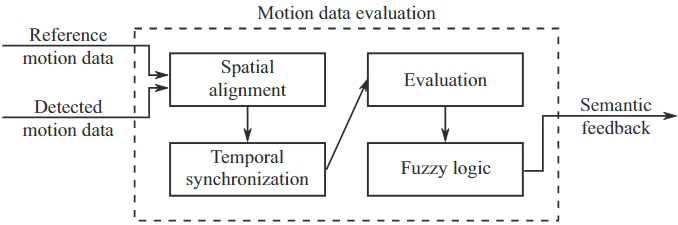
\includegraphics[width=\textwidth]{pictures/Patrona_motion_evaluation.png}
    \caption[Étapes de normalisation et d'analyse automatique du mouvement \parencite{Patrona2018MaA}]{La suite d'étapes utilisée par Patrona \textit{et al.} permet de corriger les différences spatiales et temporelles entre les mouvements de l'expert et de l'apprenant, afin de proposer une évaluation du geste en fonction des descripteurs extraits \parencite{Patrona2018MaA}.}
    \label{fig:Patrona_motion_evaluation}
\end{figure}

Dans ces travaux, la contribution de l'expert se situe en amont, lors de la formalisation de ses besoins d'observations en descripteurs calculables à partir du mouvement, voire des conseils à donner. Cependant, les données obtenues en sortie de ces systèmes doivent parfois être analysées et traduites en retour intelligible à l'apprenant par un expert. Dans tous les cas, l'expert n'intervient pas pendant le processus d'apprentissage humain. Lorsque le retour est donné par le système, les informations fournies concernent les propriétés extraites du geste : différence de positions, vitesses, \textit{etc.} Ces informations sont difficilement observables pour un apprenant sans visualisation externe, mais également dans le cas où l'apprenant ne possède pas les connaissances scientifiques requises pour être en mesure de modifier son geste pour prendre en compte les retours du système.

\section{Bilan des systèmes existants et positionnement}
Cette section présente les modalités d'usage des différentes systèmes présentés auparavant, tout en mettant en lumière leurs avantages et inconvénients par rapport à la place donnée à l'apprenant, ainsi qu'à l'enseignant, en leur sein.


Les travaux où l'analyse des gestes est réalisée par un humain sont ceux où les utilisateurs finaux (experts dans le cas d'un sytème d'assistance à l'analyse et l'évaluation du geste, ou apprenants) ont une place importante. Les systèmes dédiées à l'analyse médicale (rééducation ou suivi de maladie) nécessitent très souvent de combiner les retours proposés par le système (squelette 3D de démarche, descripteurs spécifiques extraits des parties du corps lors d'un mouvement, \textit{etc.}) au savoir de l'expert, afin de proposer un diagnostic adéquat. Dans ces cas, le système n'a pas pour objectif d'être utilisé par le patient en autonomie, car les informations fournies par le système nécessitent de disposer de la connaissance scientifique permettant d'en tirer des conclusions, et sont ainsi destinées à un expert. L'apprentissage de procédures chirurgicales au travers d'EIAH dédiés permet de proposer des entrainements sur des simulations d'opérations réelles. Dans ce cas, la connaissance experte est parfois directement intégrée au système \textit{a priori} (ordre des différents mouvement à réaliser, état successifs de l'objet à atteindre, temps total de l'opération, \textit{etc.}), ce qui permet de calculer des indicateurs précis sur le geste, correspondants aux besoins d'observation et d'analyse de l'expert. L'apprentissage du sport nécessite également très souvent un expert afin de proposer des retours compréhensibles sur le geste et exploitables par un apprenant afin de modifier son geste. Le système proposé par Burns \textit{et al.} ne propose aucun retour en lui-même, et ne sert que de support à la visualisation des mouvements de l'expert (soit sous forme de vidéo, soit sous la forme d'un squelette 3D représentant l'expert en train d'effectuer le mouvement, dans un contexte de réalité virtuelle en immersion dans un dojo virtuel). L'évaluation du geste de l'apprenant s'effectue à la fin de l'apprentissage d'un geste par l'expert, en visualisant la vidéo de l'apprenant en train d'effectuer le mouvement. L'environnement virtuel de Kora \textit{et al.}, à l'inverse des systèmes vus précédemment, ne fait intervenir l'expert que dans la phase d'enregistrement du geste cible. Le système est utilisé en autonomie totale par l'apprenant, et l'objectif est d'ajuster le geste de façon à se rapprocher le plus possible visuellement du geste cible de l'expert. Le système ne fournissant aucun conseil ni aucune métrique (indicateurs, score), l'ajustement du geste peut être difficile pour un apprenant non-expert. Enfin, le système de Yoshinaga et Soga utilise plusieurs données expertes différentes afin de proposer une comparaison du geste de l'apprenant à celui des experts les plus proches de l'apprenant au sens morphologique \parencite{Yoshinaga2015Doa}. Dans celui-ci, les experts enregistrent non seulement les mouvements cibles, mais peuvent également utiliser le système afin d'analyser le geste de l'apprenant et pour proposer un retour visuel des changements à effectuer sur le geste, en fonction des parties du corps concernées. Le système peut également être utilisé en autonomie par l'apprenant, qui ne dispose alors que de la visualisation de la superposition du mouvement cible choisi avec le sien.

Dans les systèmes où l'analyse est réalisée par un humain, l'implication de l'expert dans la conception dépend souvent de la nécessité ou non de disposer de matériels ou environnements spécifiques à la tâche considérée. Les systèmes proposant de calculer des métriques, à partir du mouvement de l'apprenant, interprétables par les experts nécessitent d'impliquer ce dernier dans le processus de conception afin d'être en mesure de satisfaire ses besoins d'observation. Les valeurs ainsi calculées à partir du geste de l'apprenant ne sont, en général, pas réutilisables dans d'autres contextes applicatifs. De plus, dans les systèmes dédiés à l'apprentissage de procédures chirurgicales, la réutilisabilité est compromise à cause de l'utilisation de matériels spécifiques (bras haptiques, par exemple). À l'inverse, les systèmes ne proposant qu'une visualisation du mouvement (soit de l'expert pendant l'apprentissage de l'apprenant, soit de l'apprenant lors de la phase d'évaluation de l'expert) sont en général très génériques et ne nécessitent ainsi pas d'intégrer l'expert dans le processus de conception, mais ne proposent en général aucune analyse sur le mouvement de l'apprenant, et n'assistent donc l'expert dans sa tâche d'évaluation que de manière marginale.

L'extraction de descripteurs à partir du geste de l'apprenant permet de fournir un ensemble de valeurs afin de l'assister dans son évaluation. Ainsi, le système de suivi de patients atteints de la maladie de Parkison proposé par Wang \textit{et al.} nécessite de faire réaliser au patient quelques mouvements types (marcher, s'asseoir, se lever), permettant ensuite de calculer des descripteurs relatifs au déplacement du patient. Les experts médicaux peuvent ensuite utiliser ces indications afin de juger de la progression du système. Il a également été pensé de manière à permettre au patient de réaliser les gestes requis à distance, afin de limiter le déplacement de ce dernier. La place du patient au sein du système se limite à effectuer les gestes demandés par l'expert ou le système. Le système de simulation d'insertion de sonde naso-gastrique développé par Choi \textit{et al.} permet de calculer la force appliquée par l'apprenant, mais également de simuler les butées contre les parois d'un modèle 3D mis à jour en temps réel \parencite{Choi2015103}. Les indicateurs extraits sont relatifs à la procédure (durée de l'opération, nombre de butées, force maximale appliquée, \textit{etc.}), et bien que leur restitution soit proposée par le système, leur analyse nécessite un expert afin d'être capable d'en tirer des conclusions sur le déroulement de l'opération, et sur les conseils à donner afin d'améliorer le geste de l'apprenant. De par la spécificité du matériel utilisé et des indicateurs calculés, le système n'est pas réutilisable dans d'autres contextes.
Les outils d'analyse automatique permettent d'évaluer le geste suivant des descripteurs géométriques, cinématiques, dynamiques et de les comparer. Cependant, des connaissances scientifiques solides sont nécessaires, tant pour l'enseignant que pour l'apprenant afin de pouvoir les interpréter. Les indicateurs utilisés peuvent parfois concerner l'objet manipulé, plutôt que le mouvement en lui-même. Dans le cas de l'EIAH développé par Pham \textit{et al.}, la trajectoire de l'outil de l'apprenant est comparée à celle de l'outil manipulé par l'expert, et cette comparaison fourni un score de similitude entre les gestes \parencite{Pham2010Tdg}. Bien qu'étant facile à interpréter pour un non-expert (la maximisation de ce score étant l'objectif), aucune indication n'est fournie sur les parties du geste à modifier afin de se rapprocher des positions de l'objet ciblées. Le même principe est utilisé par Maes \textit{et al.} dans leur système dédié à l'apprentissage de la danse, en segmentant cette fois le mouvement en plusieurs parties et en assignant un score (correspondant à la similitude des mouvements de l'apprenant par rapport à ceux de l'expert) à maximiser pour chaque partie du mouvement \parencite{Maes2012DtM}. Il n'y a toujours aucun retour proposé à l'apprenant afin d'améliorer son geste. Le système d'apprentissage de la danse proposé par Kyan \textit{et al.} utilise les mêmes concepts, mais propose en plus de cela une superposition du mouvement de l'apprenant avec celui de l'expert, afin de corriger la position de chaque partie du corps \parencite{Kyan2015ABD}. Le système proposé par Yamaoka \textit{et al.} évalue le geste du lancer de disque d'un apprenant en comparant les positions relatives des articulations entre elles à différents moment du geste. Ici, la connaissance experte est intégrée dès la conception de l'environnement, et la réutilisabilité du système dans un autre contexte nécessite une re-conception du système. De plus, les retours fournis par le système le sont en temps réel, et il n'est pas possible de rejouer le mouvement, ce qui rend plus difficile la correction et l'apprentissage du geste pour l'apprenant. L'objectif du système développé par Makio \textit{et al.} est de mettre en lumière les différences entre les gestes des apprenants et des experts, sans pour autant fournir des indications ou des retours sur les corrections à effectuer. Ainsi, l'expert et l'apprenant n'ont qu'un rôle minime au sein de la conception, et la phase de restitution en propose qu'une visualisation graphique de ces différences.

Les systèmes se basant sur le calcul d'indicateurs à partir du geste de l'apprenant permettent de s'affranchir dans une certaine mesure de la présence d'un expert pendant l'apprentissage. En effet, ils sont généralement conçus dans l'optique de proposer une évaluation du geste de l'apprenant, souvent en le comparant aux données de l'expert intégrées au préalable lors de la conception du système. Les inconvénients de ces systèmes sont le côté peu explicite des retours ainsi donnés, se limitant souvent à un simple score, et la faible réutilisabilité dans d'autres contextes, due à la nécessiter d'intégrer la connaissance experte dès la phase de conception du système.

Les outils d'analyse automatique du mouvement sont souvent conçus et développés dans l'objectif d'aider et d'assister l'expert et l'apprenant. En conséquence, la formalisation de la connaissance de l'utilisateur et de ses besoins d'observation est nécessaire, mais difficile à opérationnaliser. Le développement de ce type de systèmes a pour objectif de répondre aux défis d'adaptation au contexte d'apprentissage constitué du profil d'utilisateur (apprenant ou enseignant), du domaine d'application et de la tâche à apprendre. La généricité potentielle du système ainsi développé peut grandement varier suivant le contexte.

Les systèmes s'intéressant à la détection d'une suite d'action ordonnées au sein d'un mouvement vont dans un premier temps segmenter le mouvement en unités élémentaires, pour ensuite proposer une représentation de chacune de ces unités comparable à l'enchainement attendu par l'expert. Ces travaux nécessitent ainsi l'intégration de la connaissance experte dès la conception du système, et fait qu'ils ne sont habituellement pas génériques. Il est cependant intéressant de noter que les systèmes développés par \parencite{Mahdi2019TaE} et \parencite{Delest2019MaE} ont pris en compte la réutilisabilité du système dès la conception, et proposent ainsi des éditeurs de scénarios pédagogiques utilisables par des non-expert de la réalité virtuelle.

Enfin, les systèmes faisant usage d'apprentissage supervisé afin d'observer la similitude des mouvements de l'apprenant à ceux de l'expert nécessitent également l'intégration de la connaissance experte \textit{a priori}, afin d'utiliser l'ensemble de caractéristiques des gestes les plus pertinents afin d'obtenir la meilleure séparation possible. Le système d'évaluation de gestes développé par Patrona \textit{et al.}, bien que permettant de segmenter des gestes et de les reconnaitre sans a priori sur ces derniers \parencite{Patrona2018MaA}, nécessite une base de données de geste de comparaison suffisamment importante afin de couvrir les différents gestes possibles à reconnaitre.

Ce chapitre a présenté plusieurs techniques d'analyse du mouvement, classées en quatre catégories : (i) l'évaluation par observation, (ii) l'évaluation par analyse d'indicateurs calculables  et (iii) l'évaluation d'une séquence ordonnée d'actions (iv) l'évaluation utilisant des techniques d'apprentissage automatique. Cette étude a aussi montré l'importance de la prise en compte des connaissances et besoins d'observation de l'expert dans le processus d'observation et d'analyse, ce qui implique de placer l'expert dans le processus de conception du système informatique dédié à l'apprentissage humain.

L'analyse peut se faire à partir du geste en lui-même ou d'un découpage du geste en unités élémentaires \parencite{Despinoy2016UTS} \parencite{Yamaoka2013FoF} \parencite{Pirsiavash2014AQA}. Les mouvements sont souvent modélisés sous la forme d'un ensemble d'informations cinématiques, telles que les positions, les orientations, les vitesses, les trajectoires, la courbure du mouvement, etc. L'utilisation de tels descripteurs permet d'obtenir des informations précises à traiter. Des descripteurs fournissant des informations globales sur le geste, bien que plus facilement compréhensibles et utilisables pour l'analyse pour un humain non-expert, ne permettent pas de systématiquement mettre en évidence les différences subtiles qui permettent de juger de la qualité d'un geste.

L'apprentissage par observation et imitation est naturelle pour l'humain. Cependant, cette méthode se heurte aux capacités de perception et de connaissances de l'usager qui ne percevra pas nécessairement les propriétés du geste rendant ce dernier comme acceptable. En outre, l'analyse de toutes les caractéristiques d'un geste ainsi que leurs propriétés est difficile, tant ils dépendent des caractéristiques de la situation d'apprentissage qui demeure très contextuel. L'utilisation d'outils informatiques proposant des indicateurs quant à la performance ou la qualité du geste permet ainsi à l'expert de proposer un retour plus pertinent mais nécessitent des connaissances scientifiques solides pour être interprétés; ainsi qu'une phase de formalisation des besoins d'observation en amont.

En effet, dans le cas où les descripteurs utilisés sont extraits par un processus automatique, l'analyse en elle-même est souvent réalisée par un humain. De plus, il est difficile de proposer un retour pédagogique pertinent à l'apprenant à partir d'un processus entièrement automatisé. Dans ce cas, il faut disposer à minima d'un modèle d'expertise pédagogique, et d'un modèle de l'apprenant. Au-delà de la difficulté propre à l'extraction de descripteurs pertinents dans un cadre donné, il faut également être en mesure de fournir des indications suffisamment explicites afin que même une personne non-experte du domaine puisse être en mesure de s'auto-corriger. Bien que l'injection de la connaissance experte permet de formaliser et, par exemple, d'intégrer en amont un ensemble de conseils, ce type de systèmes est souvent réalisé de façon « \textit{ad hoc} », contextuel au domaine voire à la tâche à apprendre et peut être limité dans le cas de problèmes non-définis à l'avance.

En outre, l'outil utilisé et la connaissance experte ne se rejoignent pas forcément. Par exemple, le système de \parencite{Kyan2015ABD} propose un score pour évaluer chaque sous-partie du geste de danse, mais c'est à l'enseignant de donner les indications et corrections nécessaires afin d'améliorer le geste. Ainsi, l'outil informatique propose une pré-évaluation du geste, utilisable ou non par l'expert. L'analyse d'un geste étant matière à une certaine part de subjectivité de la part de l'expert, une étude purement automatique peut parfois ne pas être en accord avec l'avis de l'expert.

L'association des compétences de l'expert tout au long du processus d'apprentissage et d'évaluation avec l'aide possible apportée par un outil informatique est une approche qui semble être peu explorée. Un système permettant à la fois d'évaluer le geste, mais également de proposer un ensemble d'indicateurs visuels pourrait aider l'expert dans sa tâche d'évaluation lorsque l'observation n'est pas aisée. Il faut cependant qu'un tel système puisse disposer de la connaissance experte en amont, afin de pouvoir formaliser les différentes modalités du geste à analyser, et également qu'il soit en mesure de proposer des visualisations pertinentes et compréhensibles à partir des descripteurs calculés.

Le prochaine chapitre présente un système d'aide à l'observation, l'analyse et l'évaluation de gestes. Ce système est développé de manière à minimiser les travaux de réingénierie en cas de changement du geste cible à apprendre et des besoins d'observation.